El presente trabajo comprende el diseño y evaluación de un prototipo funcional de sistema multi-agente basado en MCP, orientado a la generación automatizada de documentos de SRS conformes al estándar IEEE 830-1998, a partir del procesamiento de audio de entrevistas a Product Owners.


En primer lugar, se elaborará el marco teórico mediante el estudio y análisis de literatura científica relacionada con ingeniería de requisitos, la metodología de elicitación, el estándar 
IEEE 830-1998, modelos de lenguaje de gran escala, arquitecturas multi-agente y el MCP, estableciendo los fundamentos conceptuales que sustentan el sistema propuesto.


Posteriormente, se realizará el diseño y desarrollo del sistema, el cual integrará cuatro agentes: un agente de transcripción automática del audio de la entrevista, un agente de análisis y clasificación de requisitos funcionales, un agente de enriquecimiento contextual mediante búsqueda web, y un agente generador del documento SRS estructurado conforme al estándar IEEE 830-1998. El desarrollo del sistema se gestionará mediante la metodología Scrum, organizando el trabajo en sprints con entregas incrementales que permitan una evolución controlada y adaptable del proyecto. El sistema incorporará mecanismos de persistencia en base de datos para almacenar los documentos generados y permitir su consulta y comparación futura, así como una interfaz web que permita cargar el audio de la entrevista y visualizar el documento SRS producido. Finalmente, la evaluación del sistema se realizará mediante métricas basadas en modelos de lenguaje de gran escala (LLMs) y juicio de expertos en ingeniería de requisitos, quienes validarán la conformidad, completitud y coherencia de los documentos SRS generados respecto al estándar IEEE 830-1998 generando resultados comparativos que permitan determinar la efectividad del sistema frente a la elaboración manual del documento.


Cabe señalar que el proyecto se limita al desarrollo de un prototipo funcional con fines académicos e investigativos, por lo que no contempla su integración con plataformas, ni su despliegue en entornos productivos. El entrenamiento o ajuste fino de modelos de lenguaje queda fuera del alcance, utilizándose exclusivamente modelos pre entrenados disponibles mediante API.

\newpage

\begin{figure}[H]
    \centering
    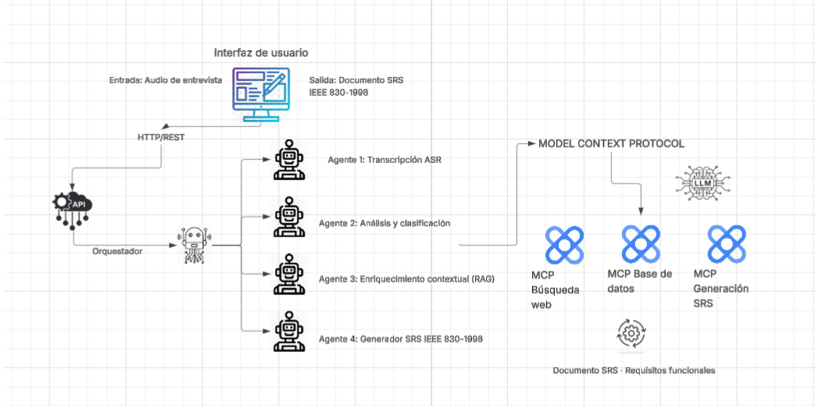
\includegraphics[width=0.9\linewidth]{ANTEPROYECTO/0.3-ALCANCE/2.png}
    \caption[Arquitectura del sistema multi-agente ] {Arquitectura del sistema multi-agente }
    \label{fig:Arquitectura}
\end{figure}


\title{Descripción del funcionamiento del sistema}
El sistema inicia cuando el usuario carga el audio de la entrevista de elicitación a través de la interfaz web. Esta interfaz se comunica con el backend mediante protocolo HTTP/REST, enviando el audio al componente central del sistema.

La petición es recibida por la API, que actúa como punto de entrada y la redirige al Agente Orquestador. Este agente es el responsable de coordinar y dirigir el flujo de trabajo entre los cuatro agentes especializados, asegurando que cada uno ejecute su tarea en el orden correcto.
Los cuatro agentes especializados operan de la siguiente manera:


El Agente 1 de Transcripción ASR recibe el audio de la entrevista y lo convierte en texto mediante reconocimiento automático de voz. El Agente 2 de Análisis y Clasificación procesa el texto transcrito para identificar y clasificar los requisitos funcionales del sistema. El Agente 3 de Enriquecimiento Contextual (RAG) amplía y enriquece el contexto de los requisitos identificados mediante búsqueda de información relevante en la web. Finalmente, el Agente 4 Generador SRS toma todos los requisitos procesados y enriquecidos para construir el documento SRS estructurado conforme al estándar IEEE 830-1998.

La comunicación entre los agentes y los servicios externos se gestiona a través del MCP, el cual conecta el sistema con tres servidores especializados: el MCP de Búsqueda Web, que provee información contextual al Agente 3; el MCP de Base de Datos, que almacena los documentos SRS generados para su consulta y comparación futura; y el MCP de Generación SRS, que apoya la construcción estructurada del documento final. Adicionalmente, todos los agentes hacen uso de un modelo de lenguaje de gran escala (LLM) para el procesamiento y generación de texto.

Como resultado final, el sistema devuelve el documento SRS completo, el cual incluye los requisitos funcionales organizados conforme al estándar IEEE 830-1998.